\documentclass{article}
\usepackage{amsmath}
\usepackage{amsfonts}
\usepackage{amssymb}
\usepackage{graphicx}

\begin{document}

The allowed region of integer solutions for the exponents \( v_0 \) and \( \bar{v}_0 \) in the ansatz for the \((m_1,m_2,m_3)=(m,m,0)\) amplitudes can be visualized as follows:

\begin{equation}
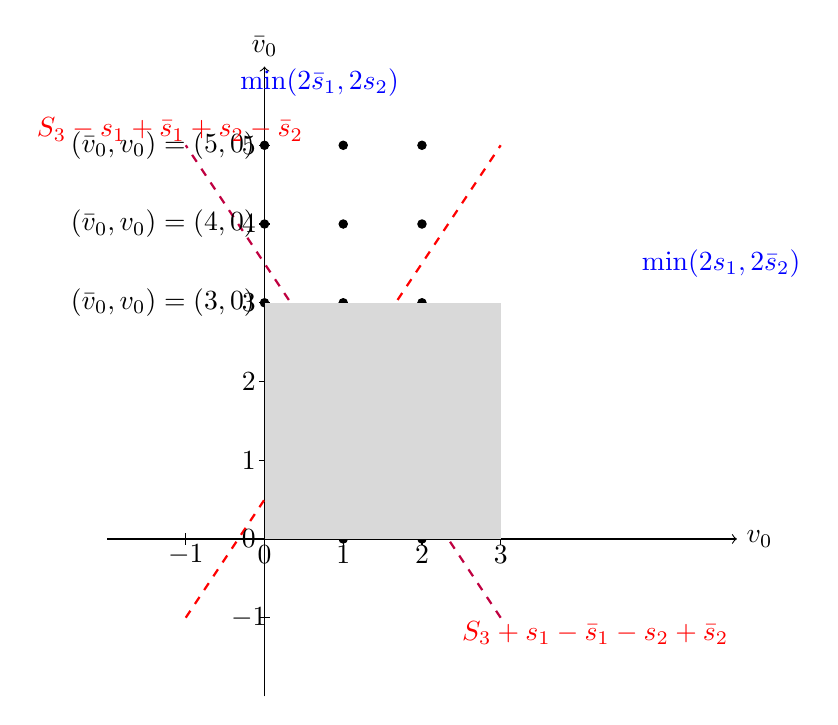
\begin{tikzpicture}[scale=1]
    \draw[->] (-2, 0) -- (6, 0) node[right] {$v_0$};
    \draw[->] (0, -2) -- (0, 6) node[above] {$\bar{v}_0$};
    
    \draw[dashed, red, thick] (-1, -1) -- (3, 5);
    \draw[dashed, purple, thick] (3, -1) -- (-1, 5);
    
    % Grid lines
    \foreach \x in {-1,...,3} {
        \draw (\x,-2pt) -- (\x,2pt);
        \node at (\x,-.2) {\(\x\)};
    }
    
    \foreach \y in {-1,...,5} {
        \draw (-2pt,\y) -- (2pt,\y);
        \node at (-.2,\y) {\(\y\)};
    }
    
    % Plot points
    \filldraw[black] (0,3) circle (1.5pt) node[left] {$(\bar{v}_0, v_0) = (3, 0)$};
    \filldraw[black] (0,4) circle (1.5pt) node[left] {$(\bar{v}_0, v_0) = (4, 0)$};
    \filldraw[black] (0,5) circle (1.5pt) node[left] {$(\bar{v}_0, v_0) = (5, 0)$};
    
    \foreach \x in {1,2} {
        \foreach \y in {0,1,2} {
            \filldraw[black] (\x,\y) circle (1.5pt);
        }
        \foreach \y in {3,4,5} {
            \filldraw[black] (\x,\y) circle (1.5pt);
        }
    }
    
    % Labels for inequalities
    \node[red] at (-1.2, 5.2) {${S_3 - s_1 + \bar{s}_1 + s_2 - \bar{s}_2}$};
    \node[red] at (4.2, -1.2) {${S_3 + s_1 - \bar{s}_1 - s_2 + \bar{s}_2}$};
    \node[blue] at (.7, 5.8) {${\min(2\bar{s}_1, 2s_2)}$};
    \node[blue] at (5.8, 3.5) {${\min(2s_1, 2\bar{s}_2)}$};
    
    % Fill the region
    \fill[gray!30] (0,0) rectangle (3,3);
\end{tikzpicture}
\end{equation}

This region represents the set of all integer pairs \((v_0, \bar{v}_0)\) that satisfy the constraints given by the inequalities.

\end{document}